\section{Code Editor}\label{section:prototypische-implementierung:code-editor}

\begin{figure}[tbp]
    \centering
    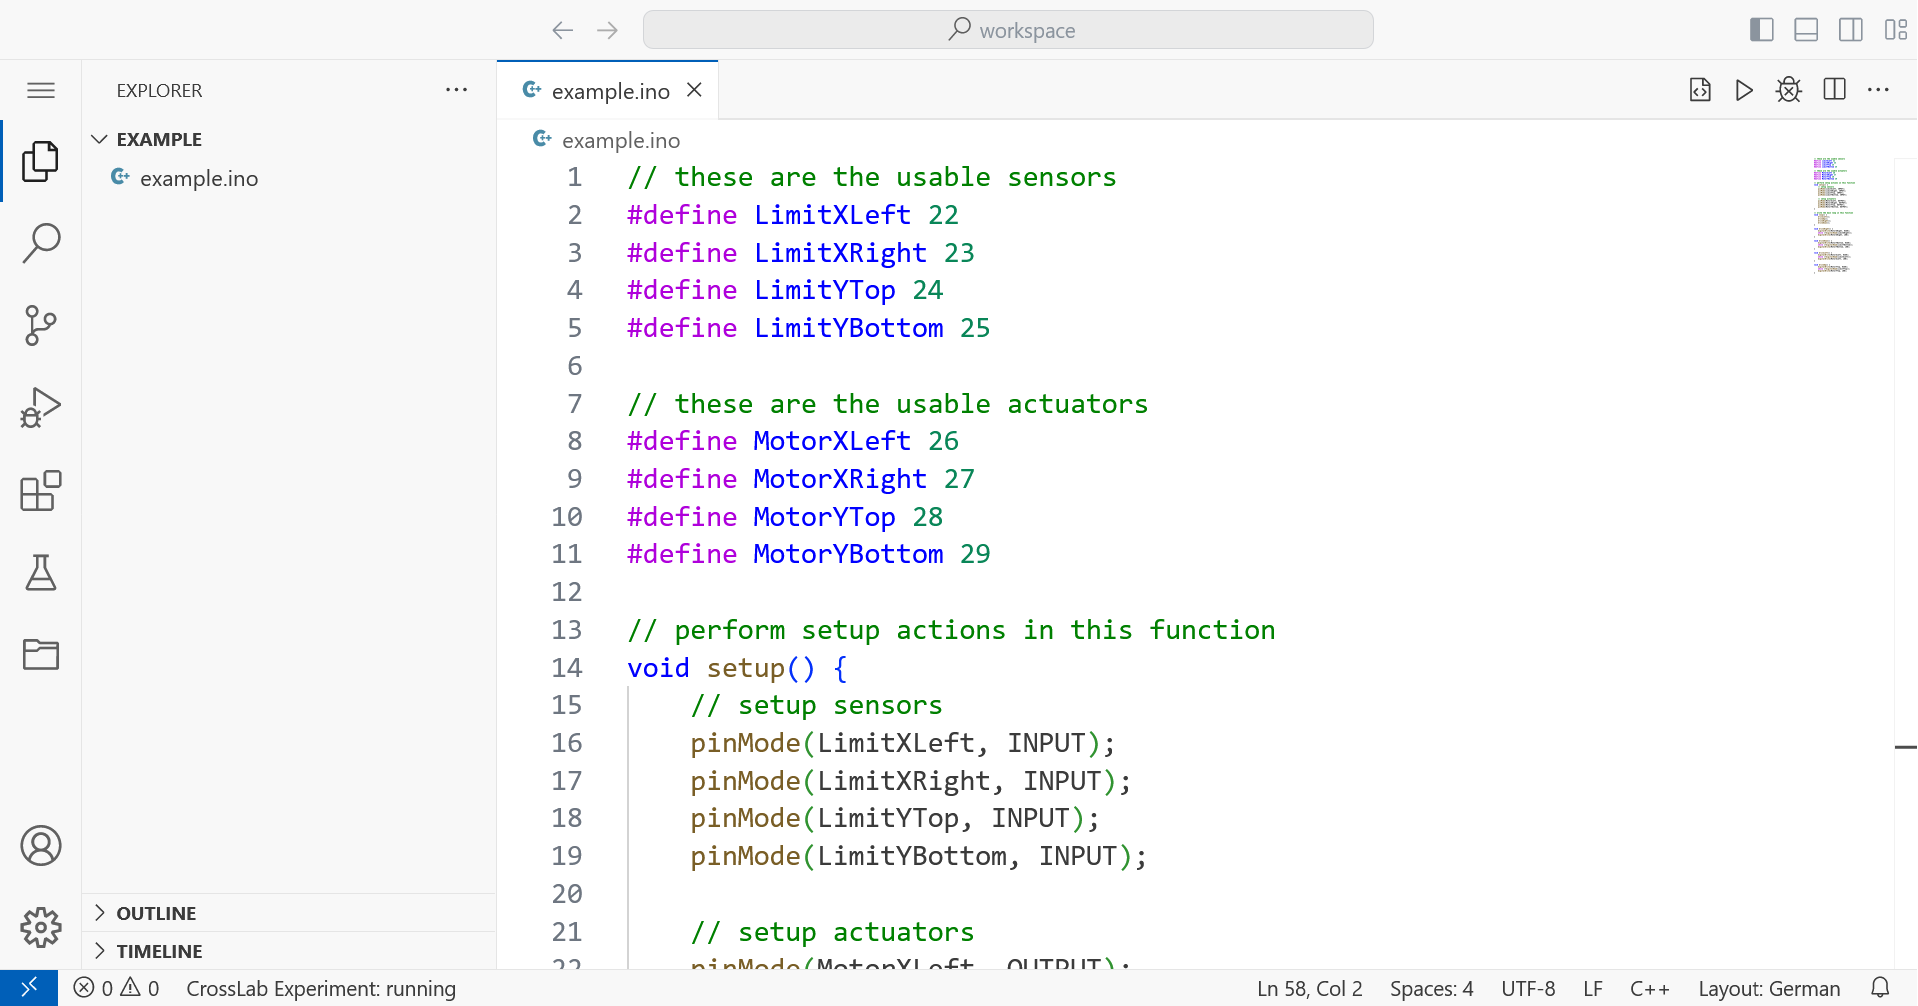
\includegraphics[trim={0 3px 0 0},clip,width=\textwidth]{images/editor.png}
    \caption{Benutzerinterface der IDE}
    \label{figure:benutzerinterface:ide}
\end{figure}

Es gibt viele verschiedene Code Editoren, die für die prototypsische Implementierung der IDE verwendet werden können. So kann ein bereits vorhandener Code Editor wie z.B. Ace \cite{noauthor_ace_nodate} oder der Monaco Editor \cite{noauthor_monaco_nodate} genutzt werden, um diese in ein eigenes Benutzerinterface einzubinden. Dies ermöglicht mit Ausnahme einer Eigenimplementierung eines Code Editors die größtmögliche Kontrolle über die Implementierung der IDE. Allerdings wird dadurch auch der Implementierungsaufwand stark erhöht. Eine weitere Option ist die Nutzung von Code Editoren, die bereits etablierte Benutzerinterfaces und Erweiterungsmöglichkeiten besitzen. Beispiele hierfür sind \ac{VSCode} \cite{noauthor_vscode_nodate}, Eclipse Theia \cite{noauthor_theia_nodate} und OpenSumi \cite{noauthor_opensumi_nodate}. Hierbei bieten Theia und OpenSumi neben der Erweiterbarkeit durch die VSCode Extension API \cite{noauthor_vscode-extension-api_nodate} auch noch weitere Schnittstellen an, die zur Erweiterung und Anpassung von grundlegenden Funktionen genutzt werden können. Durch die Nutzung bereits vorhandener und etablierter Benutzerinterfaces sowie Erweiterungsmöglichkeiten kann die Entwicklung der IDE stark vereinfacht werden. Dabei ist zu beachten, dass ggf. nicht alle erwünschten Änderungen über die angebotenen Schnittstellen umgesetzt werden können. Zudem entsteht durch die Nutzung von tiefgreifenden Schnittstellen von Theia und OpenSumi eine Bindung an das jeweilige Framework, wodurch ein späterer Wechsel auf eine andere Plattform erschwert wird. Aus diesen Gründen wird eine Implementierung über die VSCode Extension API angestrebt. Diese wird von allen drei genannten Möglichkeiten unterstützt, wodurch die entwickelte Lösung auf alle anwendbar sein sollte. Während der prototypischen Implementierung wurde \ac{VSCode} als Code Editor für die IDE verwendet. Das Benutzerinterface der entwickelten IDE ist in \autoref{figure:benutzerinterface:ide} dargestellt.
